\section{Motivation}\label{sec:motivation}

% \begin{figure}
%   \centering
%   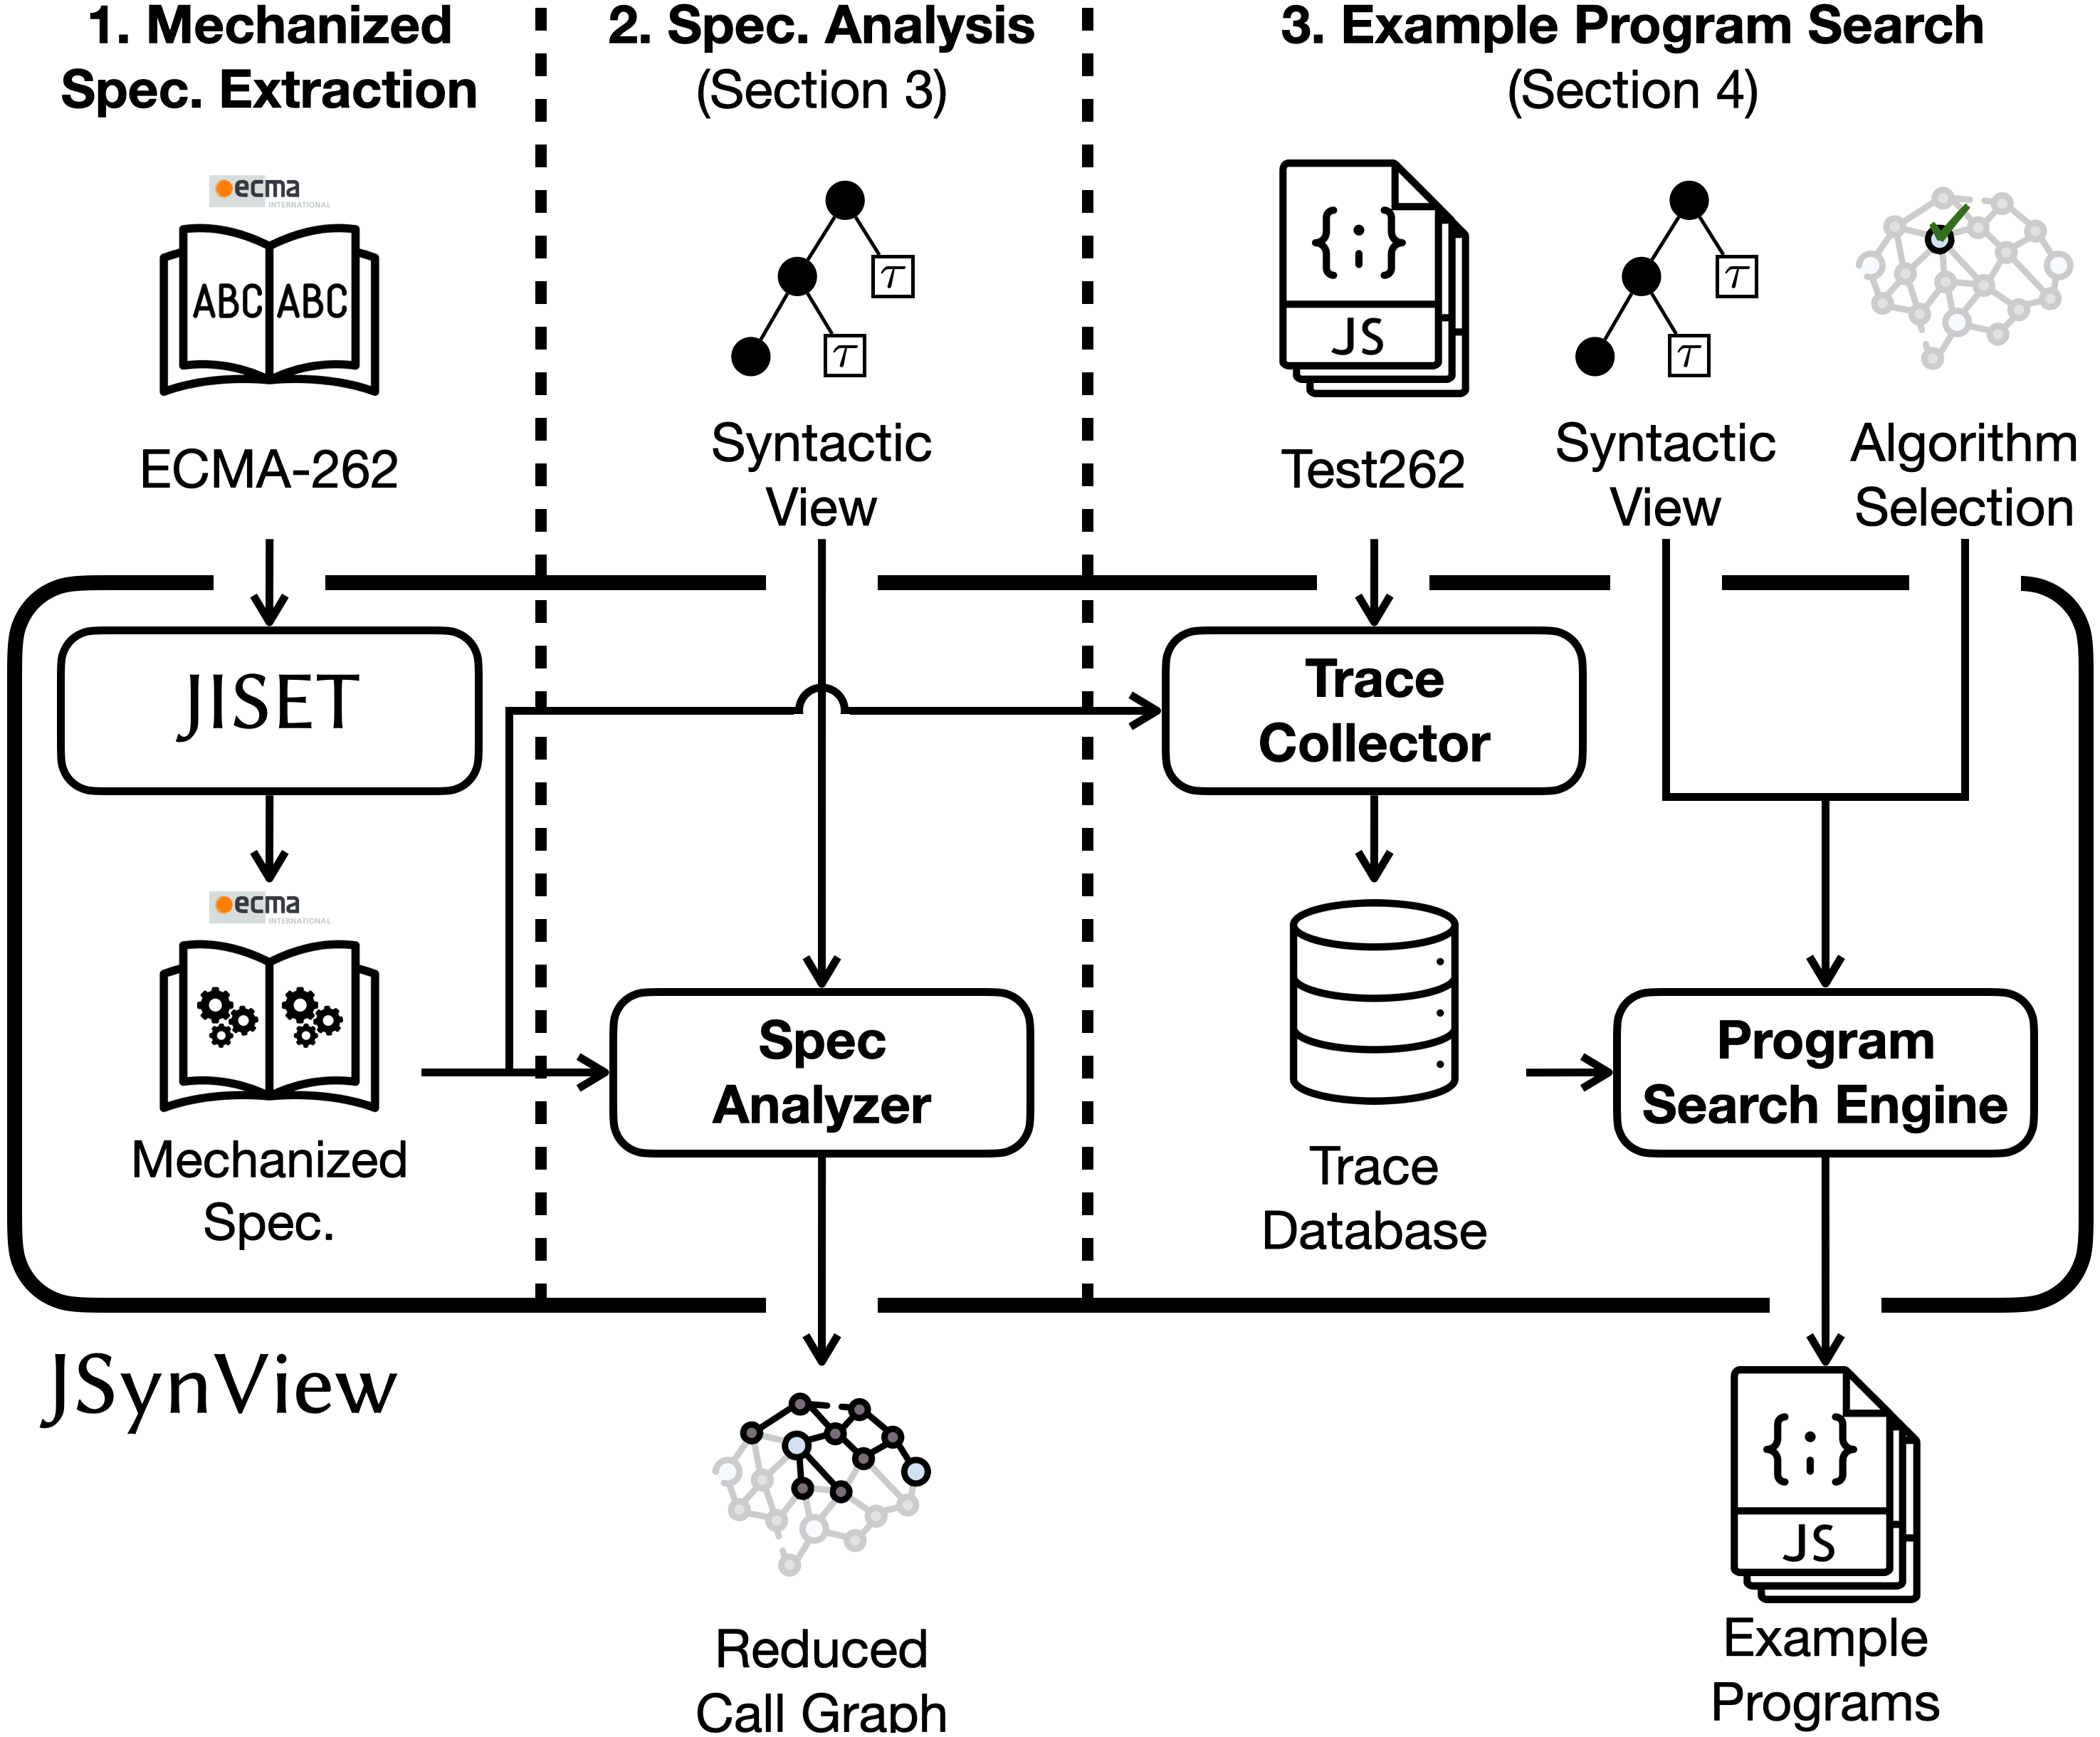
\includegraphics[width=\columnwidth]{img/overall.png}
%   \caption{The overall structure of $\tool$, a JavaScript interactive
%     specification supporting \textit{syntactic view selection} and
%   \textit{algorithm step selection}}
%   \label{fig:overall}
% \end{figure}
% 
% This section explains the overall structure of $\tool$ depicted in
% Figure~\ref{fig:overall}.
% 
% \todo

% It consists of four different modules: $\jiset$,
% \name{Step-by-Step Executor}, \name{Partial Evaluator}, and \name{Delta
% Debugger}. First, $\tool$ utilizes another tool called $\jiset$ to extract
% mechanized specification from ECMAScript.  Therefore, it is automatically
% synchronized with a given version of ECMAScript and deals with language
% semantics of the given specification.
% 
% \paragraph{Step-by-Step Execution}
% 
% dependent on a given version of ECMAScript.
% 
% extracts the JavaScript
% syntax and semantics using $\jiset$ and extracts specification types from
% ECMAScript.
% 
% \paragraph{Syntax and Semantics}
% 
% , 3) 
% 
% Our tool is a JavaScript interactive specification
% automatically synchronized with a given version of ECMAScript and supporting
% three different user interactions for better understanding of JavaScript
% language semantics. 
% 
% First, it supports \textit{step-by-step program
% execution} of a given JavaScript program with various debugging features
% 
% by strictly following the English
% sentences of the specification
% 
% by closely following the English
% sentences of the specification.
% 
% \textit{step-by-step
% execution} with various automatically synchronized with a given version of
% ECMAScript supporting k
% 
% 
% 
% which takes a specific version of ECMAScript and supports various user
% interactions for better understanding.
% automatically synchronized
% 
% depending on a given version of standard JavaScript specification, ECMAScript.
% It provides three interactions1) step-by-step execution, 2) partial
% evaluation with syntactic views, and 3) delta debugging with algorithm steps and
% JavaScript programs.
% 
% 
% official JavaScript
% dependent iwth 
% 
% takes a specific version of ECMAScript
